% Options for packages loaded elsewhere
\PassOptionsToPackage{unicode}{hyperref}
\PassOptionsToPackage{hyphens}{url}
%
\documentclass[
]{article}
\usepackage{amsmath,amssymb}
\usepackage{iftex}
\ifPDFTeX
  \usepackage[T1]{fontenc}
  \usepackage[utf8]{inputenc}
  \usepackage{textcomp} % provide euro and other symbols
\else % if luatex or xetex
  \usepackage{unicode-math} % this also loads fontspec
  \defaultfontfeatures{Scale=MatchLowercase}
  \defaultfontfeatures[\rmfamily]{Ligatures=TeX,Scale=1}
\fi
\usepackage{lmodern}
\ifPDFTeX\else
  % xetex/luatex font selection
\fi
% Use upquote if available, for straight quotes in verbatim environments
\IfFileExists{upquote.sty}{\usepackage{upquote}}{}
\IfFileExists{microtype.sty}{% use microtype if available
  \usepackage[]{microtype}
  \UseMicrotypeSet[protrusion]{basicmath} % disable protrusion for tt fonts
}{}
\makeatletter
\@ifundefined{KOMAClassName}{% if non-KOMA class
  \IfFileExists{parskip.sty}{%
    \usepackage{parskip}
  }{% else
    \setlength{\parindent}{0pt}
    \setlength{\parskip}{6pt plus 2pt minus 1pt}}
}{% if KOMA class
  \KOMAoptions{parskip=half}}
\makeatother
\usepackage{xcolor}
\usepackage[margin=1in]{geometry}
\usepackage{color}
\usepackage{fancyvrb}
\newcommand{\VerbBar}{|}
\newcommand{\VERB}{\Verb[commandchars=\\\{\}]}
\DefineVerbatimEnvironment{Highlighting}{Verbatim}{commandchars=\\\{\}}
% Add ',fontsize=\small' for more characters per line
\usepackage{framed}
\definecolor{shadecolor}{RGB}{248,248,248}
\newenvironment{Shaded}{\begin{snugshade}}{\end{snugshade}}
\newcommand{\AlertTok}[1]{\textcolor[rgb]{0.94,0.16,0.16}{#1}}
\newcommand{\AnnotationTok}[1]{\textcolor[rgb]{0.56,0.35,0.01}{\textbf{\textit{#1}}}}
\newcommand{\AttributeTok}[1]{\textcolor[rgb]{0.13,0.29,0.53}{#1}}
\newcommand{\BaseNTok}[1]{\textcolor[rgb]{0.00,0.00,0.81}{#1}}
\newcommand{\BuiltInTok}[1]{#1}
\newcommand{\CharTok}[1]{\textcolor[rgb]{0.31,0.60,0.02}{#1}}
\newcommand{\CommentTok}[1]{\textcolor[rgb]{0.56,0.35,0.01}{\textit{#1}}}
\newcommand{\CommentVarTok}[1]{\textcolor[rgb]{0.56,0.35,0.01}{\textbf{\textit{#1}}}}
\newcommand{\ConstantTok}[1]{\textcolor[rgb]{0.56,0.35,0.01}{#1}}
\newcommand{\ControlFlowTok}[1]{\textcolor[rgb]{0.13,0.29,0.53}{\textbf{#1}}}
\newcommand{\DataTypeTok}[1]{\textcolor[rgb]{0.13,0.29,0.53}{#1}}
\newcommand{\DecValTok}[1]{\textcolor[rgb]{0.00,0.00,0.81}{#1}}
\newcommand{\DocumentationTok}[1]{\textcolor[rgb]{0.56,0.35,0.01}{\textbf{\textit{#1}}}}
\newcommand{\ErrorTok}[1]{\textcolor[rgb]{0.64,0.00,0.00}{\textbf{#1}}}
\newcommand{\ExtensionTok}[1]{#1}
\newcommand{\FloatTok}[1]{\textcolor[rgb]{0.00,0.00,0.81}{#1}}
\newcommand{\FunctionTok}[1]{\textcolor[rgb]{0.13,0.29,0.53}{\textbf{#1}}}
\newcommand{\ImportTok}[1]{#1}
\newcommand{\InformationTok}[1]{\textcolor[rgb]{0.56,0.35,0.01}{\textbf{\textit{#1}}}}
\newcommand{\KeywordTok}[1]{\textcolor[rgb]{0.13,0.29,0.53}{\textbf{#1}}}
\newcommand{\NormalTok}[1]{#1}
\newcommand{\OperatorTok}[1]{\textcolor[rgb]{0.81,0.36,0.00}{\textbf{#1}}}
\newcommand{\OtherTok}[1]{\textcolor[rgb]{0.56,0.35,0.01}{#1}}
\newcommand{\PreprocessorTok}[1]{\textcolor[rgb]{0.56,0.35,0.01}{\textit{#1}}}
\newcommand{\RegionMarkerTok}[1]{#1}
\newcommand{\SpecialCharTok}[1]{\textcolor[rgb]{0.81,0.36,0.00}{\textbf{#1}}}
\newcommand{\SpecialStringTok}[1]{\textcolor[rgb]{0.31,0.60,0.02}{#1}}
\newcommand{\StringTok}[1]{\textcolor[rgb]{0.31,0.60,0.02}{#1}}
\newcommand{\VariableTok}[1]{\textcolor[rgb]{0.00,0.00,0.00}{#1}}
\newcommand{\VerbatimStringTok}[1]{\textcolor[rgb]{0.31,0.60,0.02}{#1}}
\newcommand{\WarningTok}[1]{\textcolor[rgb]{0.56,0.35,0.01}{\textbf{\textit{#1}}}}
\usepackage{graphicx}
\makeatletter
\def\maxwidth{\ifdim\Gin@nat@width>\linewidth\linewidth\else\Gin@nat@width\fi}
\def\maxheight{\ifdim\Gin@nat@height>\textheight\textheight\else\Gin@nat@height\fi}
\makeatother
% Scale images if necessary, so that they will not overflow the page
% margins by default, and it is still possible to overwrite the defaults
% using explicit options in \includegraphics[width, height, ...]{}
\setkeys{Gin}{width=\maxwidth,height=\maxheight,keepaspectratio}
% Set default figure placement to htbp
\makeatletter
\def\fps@figure{htbp}
\makeatother
\setlength{\emergencystretch}{3em} % prevent overfull lines
\providecommand{\tightlist}{%
  \setlength{\itemsep}{0pt}\setlength{\parskip}{0pt}}
\setcounter{secnumdepth}{-\maxdimen} % remove section numbering
\ifLuaTeX
  \usepackage{selnolig}  % disable illegal ligatures
\fi
\usepackage{bookmark}
\IfFileExists{xurl.sty}{\usepackage{xurl}}{} % add URL line breaks if available
\urlstyle{same}
\hypersetup{
  hidelinks,
  pdfcreator={LaTeX via pandoc}}

\author{}
\date{\vspace{-2.5em}}

\begin{document}

\section{Clustering Analysis of Bee Eye
Data}\label{clustering-analysis-of-bee-eye-data}

\subsubsection{Loading Libraries}\label{loading-libraries}

\begin{Shaded}
\begin{Highlighting}[]
\NormalTok{packages }\OtherTok{\textless{}{-}} \FunctionTok{c}\NormalTok{(}\StringTok{"tidyverse"}\NormalTok{, }\StringTok{"cluster"}\NormalTok{, }\StringTok{"dendextend"}\NormalTok{, }\StringTok{"factoextra"}\NormalTok{, }\StringTok{"gridExtra"}\NormalTok{, }\StringTok{"writexl"}\NormalTok{)}
\CommentTok{\#lapply(packages, library, character.only = TRUE)}
\end{Highlighting}
\end{Shaded}

\subsubsection{Function to perform hierarchical
clustering}\label{function-to-perform-hierarchical-clustering}

\begin{Shaded}
\begin{Highlighting}[]
\NormalTok{perform\_hierarchical\_clustering }\OtherTok{\textless{}{-}} \ControlFlowTok{function}\NormalTok{(data, }\AttributeTok{method =} \StringTok{"average"}\NormalTok{, }\AttributeTok{k =} \DecValTok{3}\NormalTok{) \{}
\NormalTok{  distance }\OtherTok{\textless{}{-}} \FunctionTok{dist}\NormalTok{(data, }\AttributeTok{method =} \StringTok{"euclidean"}\NormalTok{)}
\NormalTok{  cluster }\OtherTok{\textless{}{-}} \FunctionTok{hclust}\NormalTok{(distance, }\AttributeTok{method =}\NormalTok{ method)}
  \FunctionTok{plot}\NormalTok{(cluster, }\AttributeTok{cex =} \FloatTok{0.6}\NormalTok{, }\AttributeTok{hang =} \SpecialCharTok{{-}}\DecValTok{1}\NormalTok{)}
  \FunctionTok{rect.hclust}\NormalTok{(cluster, }\AttributeTok{k =}\NormalTok{ k)  }\CommentTok{\# Highlight groups}
  \FunctionTok{return}\NormalTok{(cluster)}
\NormalTok{\}}
\end{Highlighting}
\end{Shaded}

\subsubsection{Function to generate and plot clusters for
K-means}\label{function-to-generate-and-plot-clusters-for-k-means}

\begin{Shaded}
\begin{Highlighting}[]
\NormalTok{generate\_kmeans\_clusters }\OtherTok{\textless{}{-}} \ControlFlowTok{function}\NormalTok{(data, centers, title) \{}
\NormalTok{  kmeans\_result }\OtherTok{\textless{}{-}} \FunctionTok{kmeans}\NormalTok{(data, }\AttributeTok{centers =}\NormalTok{ centers)}
\NormalTok{  plot }\OtherTok{\textless{}{-}} \FunctionTok{fviz\_cluster}\NormalTok{(kmeans\_result, }\AttributeTok{geom =} \StringTok{"point"}\NormalTok{, }\AttributeTok{data =}\NormalTok{ data) }\SpecialCharTok{+} \FunctionTok{ggtitle}\NormalTok{(title)}
  \FunctionTok{return}\NormalTok{(}\FunctionTok{list}\NormalTok{(}\AttributeTok{model =}\NormalTok{ kmeans\_result, }\AttributeTok{plot =}\NormalTok{ plot))}
\NormalTok{\}}
\end{Highlighting}
\end{Shaded}

\subsubsection{Function to visualize elbow and silhouette
methods}\label{function-to-visualize-elbow-and-silhouette-methods}

\begin{Shaded}
\begin{Highlighting}[]
\NormalTok{evaluate\_clusters }\OtherTok{\textless{}{-}} \ControlFlowTok{function}\NormalTok{(data, clustering\_function) \{}
  \CommentTok{\# Elbow method}
\NormalTok{  elbow\_plot }\OtherTok{\textless{}{-}} \FunctionTok{fviz\_nbclust}\NormalTok{(data, clustering\_function, }\AttributeTok{method =} \StringTok{"wss"}\NormalTok{)}
  \FunctionTok{print}\NormalTok{(elbow\_plot)  }\CommentTok{\# Exibe o gráfico do Elbow}
  
  \CommentTok{\# Silhouette method}
\NormalTok{  silhouette\_plot }\OtherTok{\textless{}{-}} \FunctionTok{fviz\_nbclust}\NormalTok{(data, clustering\_function, }\AttributeTok{method =} \StringTok{"silhouette"}\NormalTok{)}
  \FunctionTok{print}\NormalTok{(silhouette\_plot)  }\CommentTok{\# Exibe o gráfico do Silhouette}
\NormalTok{\}}
\end{Highlighting}
\end{Shaded}

\subsubsection{Function to calculate descriptive statistics for
clusters}\label{function-to-calculate-descriptive-statistics-for-clusters}

\begin{Shaded}
\begin{Highlighting}[]
\NormalTok{calculate\_means\_by\_group }\OtherTok{\textless{}{-}} \ControlFlowTok{function}\NormalTok{(data, cluster\_column) \{}
\NormalTok{  summary }\OtherTok{\textless{}{-}}\NormalTok{ data }\SpecialCharTok{\%\textgreater{}\%}
    \FunctionTok{group\_by}\NormalTok{(}\SpecialCharTok{!!}\FunctionTok{sym}\NormalTok{(cluster\_column)) }\SpecialCharTok{\%\textgreater{}\%}
    \FunctionTok{summarise}\NormalTok{(}\AttributeTok{n =} \FunctionTok{n}\NormalTok{(),}
              \AttributeTok{ff =} \FunctionTok{mean}\NormalTok{(ff),}
              \AttributeTok{df =} \FunctionTok{mean}\NormalTok{(df),}
              \AttributeTok{vf =} \FunctionTok{mean}\NormalTok{(vf),}
              \AttributeTok{co =} \FunctionTok{mean}\NormalTok{(co),}
              \AttributeTok{nf =} \FunctionTok{mean}\NormalTok{(nf),}
              \AttributeTok{nfa =} \FunctionTok{mean}\NormalTok{(nfa),}
              \AttributeTok{ea =} \FunctionTok{mean}\NormalTok{(ea),}
              \AttributeTok{di =} \FunctionTok{mean}\NormalTok{(di))}
  \FunctionTok{return}\NormalTok{(summary)}
\NormalTok{\}}
\end{Highlighting}
\end{Shaded}

\subsection{Hierarchical clustering}\label{hierarchical-clustering}

\subsubsection{loagind data}\label{loagind-data}

\begin{Shaded}
\begin{Highlighting}[]
\NormalTok{eyes }\OtherTok{\textless{}{-}} \FunctionTok{read.table}\NormalTok{(}\StringTok{"F:/open\_git/bee\_eyes/data/eyes\_df.txt"}\NormalTok{, }\AttributeTok{header =} \ConstantTok{TRUE}\NormalTok{, }\AttributeTok{sep =} \StringTok{"}\SpecialCharTok{\textbackslash{}t}\StringTok{"}\NormalTok{)}
\end{Highlighting}
\end{Shaded}

\subsubsection{Transforming species names into row
names}\label{transforming-species-names-into-row-names}

\paragraph{Adding a suffix to ensure line names are
unique}\label{adding-a-suffix-to-ensure-line-names-are-unique}

\begin{Shaded}
\begin{Highlighting}[]
\FunctionTok{row.names}\NormalTok{(eyes) }\OtherTok{\textless{}{-}} \FunctionTok{make.unique}\NormalTok{(}\FunctionTok{as.character}\NormalTok{(eyes[, }\DecValTok{1}\NormalTok{]))}
\NormalTok{eyes }\OtherTok{\textless{}{-}}\NormalTok{ eyes[, }\SpecialCharTok{{-}}\DecValTok{1}\NormalTok{]}
\end{Highlighting}
\end{Shaded}

\section{Standardizing variables}\label{standardizing-variables}

\begin{Shaded}
\begin{Highlighting}[]
\NormalTok{eyes\_standardized }\OtherTok{\textless{}{-}} \FunctionTok{scale}\NormalTok{(eyes[, }\DecValTok{2}\SpecialCharTok{:}\DecValTok{7}\NormalTok{])}
\end{Highlighting}
\end{Shaded}

\subsection{Performing hierarchical
clustering}\label{performing-hierarchical-clustering}

\begin{Shaded}
\begin{Highlighting}[]
\NormalTok{cluster\_hierarchical }\OtherTok{\textless{}{-}} \FunctionTok{perform\_hierarchical\_clustering}\NormalTok{(eyes\_standardized, }\AttributeTok{method =} \StringTok{"average"}\NormalTok{, }\AttributeTok{k =} \DecValTok{3}\NormalTok{)}
\end{Highlighting}
\end{Shaded}

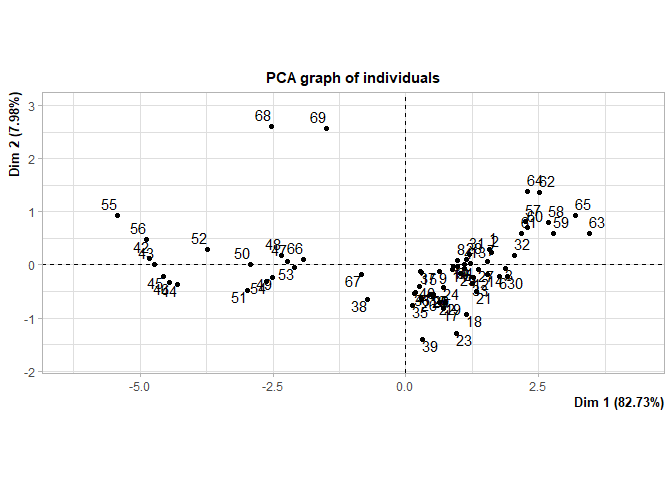
\includegraphics{cluster_bee_eyes_files/figure-latex/unnamed-chunk-10-1.pdf}

\subsubsection{Elbow and Silhouette methods for hierarchical
clustering}\label{elbow-and-silhouette-methods-for-hierarchical-clustering}

\begin{Shaded}
\begin{Highlighting}[]
\FunctionTok{evaluate\_clusters}\NormalTok{(eyes\_standardized, hcut)}
\end{Highlighting}
\end{Shaded}

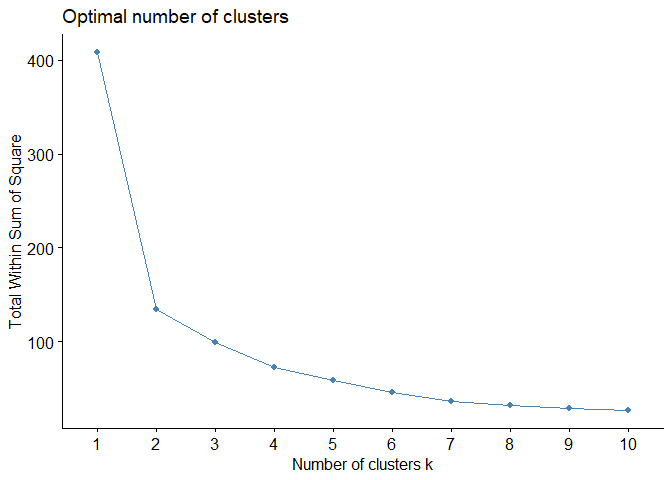
\includegraphics{cluster_bee_eyes_files/figure-latex/unnamed-chunk-11-1.pdf}
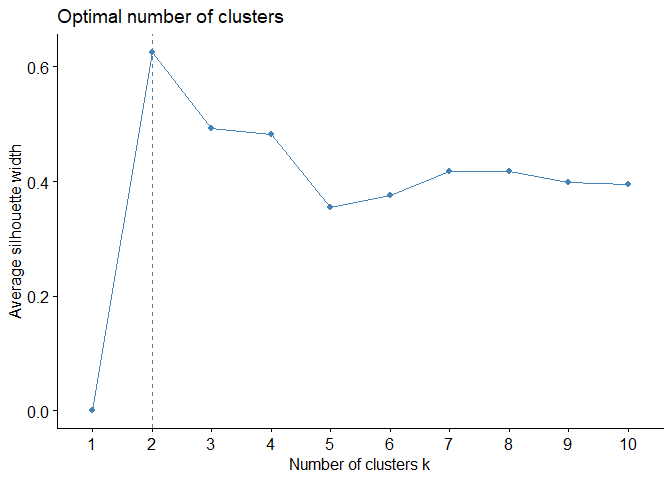
\includegraphics{cluster_bee_eyes_files/figure-latex/unnamed-chunk-11-2.pdf}

\subsubsection{Creating 3 groups of
clusters}\label{creating-3-groups-of-clusters}

\begin{Shaded}
\begin{Highlighting}[]
\NormalTok{group\_eyes3 }\OtherTok{\textless{}{-}} \FunctionTok{cutree}\NormalTok{(cluster\_hierarchical, }\AttributeTok{k =} \DecValTok{3}\NormalTok{)}
\NormalTok{eyes}\SpecialCharTok{$}\NormalTok{group\_eyes3 }\OtherTok{\textless{}{-}}\NormalTok{ group\_eyes3}
\end{Highlighting}
\end{Shaded}

\paragraph{Saving cluster results to an Excel
file}\label{saving-cluster-results-to-an-excel-file}

\begin{Shaded}
\begin{Highlighting}[]
\FunctionTok{write\_xlsx}\NormalTok{(eyes, }\StringTok{"F:/open\_git/bee\_eyes/results/clustereyes\_average\_r\_.xlsx"}\NormalTok{)}
\end{Highlighting}
\end{Shaded}

\subsubsection{Performing descriptive analysis by
group}\label{performing-descriptive-analysis-by-group}

\begin{Shaded}
\begin{Highlighting}[]
\NormalTok{mediagroup }\OtherTok{\textless{}{-}} \FunctionTok{calculate\_means\_by\_group}\NormalTok{(eyes, }\StringTok{"group\_eyes3"}\NormalTok{)}
\FunctionTok{print}\NormalTok{(mediagroup)}
\end{Highlighting}
\end{Shaded}

\begin{verbatim}
## # A tibble: 3 x 10
##   group_eyes3     n    ff    df    vf    co    nf   nfa    ea    di
##         <int> <int> <dbl> <dbl> <dbl> <dbl> <dbl> <dbl> <dbl> <dbl>
## 1           1    51  34.9  27.5  34.5  421. 4327. 1081.  4.11  3.11
## 2           2    16  22.8  17.5  23.6  218. 3834. 2387.  1.78  2.24
## 3           3     2  19.5  21    19.6  464. 7819  2010.  3.89  4.75
\end{verbatim}

\subsection{Non-hierarchical
clustering}\label{non-hierarchical-clustering}

\subsubsection{Running K-Means for multiple centers and
plotting}\label{running-k-means-for-multiple-centers-and-plotting}

\begin{Shaded}
\begin{Highlighting}[]
\NormalTok{kmeans\_results }\OtherTok{\textless{}{-}} \FunctionTok{list}\NormalTok{()}
\ControlFlowTok{for}\NormalTok{ (k }\ControlFlowTok{in} \DecValTok{2}\SpecialCharTok{:}\DecValTok{5}\NormalTok{) \{}
\NormalTok{  result }\OtherTok{\textless{}{-}} \FunctionTok{generate\_kmeans\_clusters}\NormalTok{(eyes\_standardized, }\AttributeTok{centers =}\NormalTok{ k, }\AttributeTok{title =} \FunctionTok{paste}\NormalTok{(}\StringTok{"k ="}\NormalTok{, k))}
\NormalTok{  kmeans\_results[[}\FunctionTok{paste0}\NormalTok{(}\StringTok{"k"}\NormalTok{, k)]] }\OtherTok{\textless{}{-}}\NormalTok{ result}
\NormalTok{\}}
\end{Highlighting}
\end{Shaded}

\subsubsection{Arranging all K-Means cluster plots on the same
screen}\label{arranging-all-k-means-cluster-plots-on-the-same-screen}

\begin{Shaded}
\begin{Highlighting}[]
\FunctionTok{grid.arrange}\NormalTok{(kmeans\_results}\SpecialCharTok{$}\NormalTok{k2}\SpecialCharTok{$}\NormalTok{plot, kmeans\_results}\SpecialCharTok{$}\NormalTok{k3}\SpecialCharTok{$}\NormalTok{plot,}
\NormalTok{             kmeans\_results}\SpecialCharTok{$}\NormalTok{k4}\SpecialCharTok{$}\NormalTok{plot, kmeans\_results}\SpecialCharTok{$}\NormalTok{k5}\SpecialCharTok{$}\NormalTok{plot, }\AttributeTok{nrow =} \DecValTok{2}\NormalTok{)}
\end{Highlighting}
\end{Shaded}

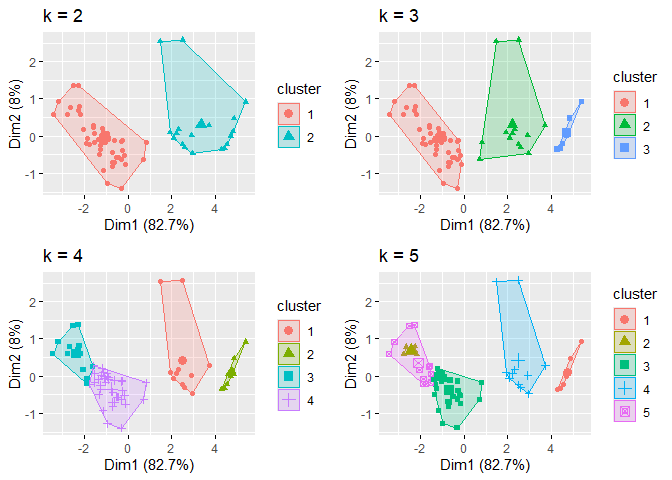
\includegraphics{cluster_bee_eyes_files/figure-latex/unnamed-chunk-16-1.pdf}

\end{document}
